% Template created by Karol Kozioł (www.karol-koziol.net) for ShareLaTeX

\documentclass[a4paper,9pt]{extarticle}
\usepackage[utf8]{inputenc}
\usepackage[T1]{fontenc}
\usepackage{graphicx}
\usepackage[table]{xcolor}
\usepackage{colortbl}
\usepackage{tikz}
\usepackage{hyperref}
\usepackage{units}
\usepackage{xspace}
 \usepackage{longtable}

\usepackage{amsmath,amssymb,textcomp}
\everymath{\displaystyle}

\usepackage{times}
\renewcommand\familydefault{\sfdefault}
\usepackage{tgheros}
\usepackage[defaultmono,scale=0.85]{droidmono}

\usepackage{multicol}
\setlength{\columnseprule}{0pt}
\setlength{\columnsep}{20.0pt}


\usepackage{geometry}
\geometry{
a4paper,
total={210mm,297mm},
left=10mm,right=10mm,top=10mm,bottom=15mm}

\linespread{1.3}

\makeatletter
\newcommand\footnoteref[1]{\protected@xdef\@thefnmark{\ref{#1}}\@footnotemark}
\makeatother

% custom title
\makeatletter
\renewcommand*{\maketitle}{%
\noindent
\begin{minipage}{0.4\textwidth}

\begin{tikzpicture}
\node[rectangle,rounded corners=6pt,inner sep=10pt,fill=blue!50!black,text width= 0.95\textwidth] {\color{white}\Huge \@title};
\end{tikzpicture}
\end{minipage}
\hfill
\begin{minipage}{0.55\textwidth}
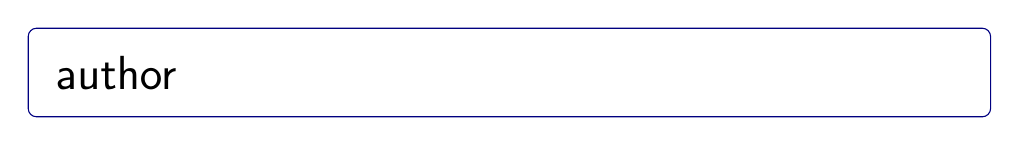
\begin{tikzpicture}
\node[rectangle,rounded corners=3pt,inner sep=10pt,draw=blue!50!black,text width= 0.95\textwidth] {\LARGE \@author};
\end{tikzpicture}
\end{minipage}
\bigskip\bigskip
}%
\makeatother

% custom section
\usepackage[explicit]{titlesec}
\newcommand*\sectionlabel{}
\titleformat{\section}
  {\gdef\sectionlabel{}
   \normalfont\sffamily\Large\bfseries\scshape}
  {\gdef\sectionlabel{\thesection\ }}{0pt}
  {
\noindent
\begin{tikzpicture}
\node[rectangle,rounded corners=3pt,inner sep=4pt,fill=blue!50!black,text width= 0.95\columnwidth] {\color{white}\sectionlabel#1};
\end{tikzpicture}
  }
\titlespacing*{\section}{0pt}{15pt}{10pt}


% custom footer
\usepackage{fancyhdr}
\makeatletter
\pagestyle{fancy}
\fancyhead{}
\fancyfoot[C]{\footnotesize \textcopyright\ \@date\ \ \@author}
\renewcommand{\headrulewidth}{0pt}
\renewcommand{\footrulewidth}{0pt}
\makeatother


\title{OpenSwarm Cheat Sheet}
\author{Stefan M. Trenkwalder, University of Sheffield}
\date{2017}


\newcommand{\uintt}{\href{http://openswarm.org/os-doc/d6/dc2/definitions\_8h.html\#a1445ebbbf93d62972255ec5e89a5ab01}{\texttt{uint}}\xspace}
\newcommand{\sintt}{\href{http://openswarm.org/os-doc/d6/dc2/definitions\_8h.html\#a0cfd70ce9210301c9c924b2f8dce5ab3}{\texttt{sint}}\xspace}
\newcommand{\uintE}{\href{http://openswarm.org/os-doc/d6/dc2/definitions\_8h.html\#adde6aaee8457bee49c2a92621fe22b79}{\texttt{uint8}}\xspace}
\newcommand{\sintE}{\href{http://openswarm.org/os-doc/d6/dc2/definitions\_8h.html\#a1a6408291ee3cfd0760a61ac64084154}{\texttt{sint8}}\xspace}
\newcommand{\uintS}{\href{http://openswarm.org/os-doc/d6/dc2/definitions\_8h.html\#a05f6b0ae8f6a6e135b0e290c25fe0e4e}{\texttt{uint16}}\xspace}
\newcommand{\sintS}{\href{http://openswarm.org/os-doc/d6/dc2/definitions\_8h.html\#a74df79fde3c518e55b29ce6360a9c76e}{\texttt{sint16}}\xspace}
\newcommand{\uintT}{\href{http://openswarm.org/os-doc/d6/dc2/definitions\_8h.html\#a1134b580f8da4de94ca6b1de4d37975e}{\texttt{uint32}}\xspace}
\newcommand{\sintT}{\href{http://openswarm.org/os-doc/d6/dc2/definitions\_8h.html\#a0573de65958b4fda3a0460ed417dafb8}{\texttt{sint32}}\xspace}
\newcommand{\syscolour}{\href{http://openswarm.org/os-doc/d6/dc2/definitions\_8h.html\#a305962be90b6e5c8f0dd0b7b48604f26}{\texttt{sys\_colour}}\xspace}
\newcommand{\syseventdata}{\href{http://openswarm.org/os-doc/d7/d0c/structsys__event__data.html}{\texttt{sys\_event\_data}}\xspace}

\newcommand{\pEventHandlerFunction}{\href{http://openswarm.org/os-doc/db/dd2/events\_8h.html\#a3db5730a7fed6827a4c46ff3fae3e55b}{\texttt{pEventHandlerFunction}}\xspace}
\newcommand{\pConditionFunction}{\href{http://openswarm.org/os-doc/db/dd2/events\_8h.html\#a653a4a4b7d9f5a65e1415365267a9d9e}{\texttt{pConditionFunction}}\xspace}
\newcommand{\pFunction}{\href{http://openswarm.org/os-doc/d6/dc2/definitions\_8h.html\#aed53e618f2025481fbe48a5098f70079}{\texttt{pFunction}}\xspace}

\begin{document}
  \rowcolors{2}{blue!25}{blue!5}

\maketitle

%\begin{multicols*}{2}


\section{Basic}

These functions are required to initialise and run OpenSwarm.

\begin{center}

\begin{tabular}{lc}
    \rowcolor{blue!50}
    Description				&	Function Name\\
    Initialise OpenSwarm  	& 	\href{http://openswarm.org/os-doc/dc/db2/system_8h.html#a9cfaef0a7af7eea16e065c481662eaa4}{\texttt{Sys\_Init\_Kernel()}} \\
    Start OpenSwarm	      	& 	\href{http://openswarm.org/os-doc/dc/db2/system_8h.html#a9cfaef0a7af7eea16e065c481662eaa4}{\texttt{Sys\_Start\_Kernel()}}
\end{tabular}

\end{center}

\section{Threads}

The following functions describe how threads can be used and controlled.

\begin{center}
\begin{tabular}{lc}
    \rowcolor{blue!50}
    Description				&	Function Name\\
    Create a new thread  	& 	\href{http://openswarm.org/os-doc/da/d14/process__Management_8c.html#a0833f904557c4c9b39b4cf5c1e43586f}{\texttt{Sys\_Start\_Process}(\pFunction function)}
\end{tabular}\\
\end{center}
    
To control the work flow of a thread, the following functions can be used (Note that a critical section is a sequence of code that cannot be interrupted by any interrupt): 
 
\begin{center}   
\begin{tabular}{lc}
    \rowcolor{blue!50}
    Description				&	Function Name\\
    Wait for an event  	& 	\syseventdata *\href{http://openswarm.org/os-doc/da/d14/process__Management_8c.html#a4b45be80626e64bb659b16e5dabcfc1d}{\texttt{Sys\_Wait\_For\_Event}(\uintt eventID)}\\
    Wait for a condition  	& 	\syseventdata *\href{http://openswarm.org/os-doc/da/d14/process__Management_8c.html#a4b45be80626e64bb659b16e5dabcfc1d}{\texttt{Sys\_Wait\_For\_Condition}(\uintt eventID, \pConditionFunction c)}\\
    Start a Critical Section  	& 	\href{http://openswarm.org/os-doc/da/d14/process__Management_8c.html#a355c5fe8c9052d6bd2ddd7ff8e8783f0}{\texttt{Sys\_Start\_AtomicSection}()}\\
    Stop a Critical Section  	& 	\href{http://openswarm.org/os-doc/dd/de5/process__Management_8h.html#ae1b0a2e19c666539afa53d571c914d6e}{\texttt{Sys\_End\_AtomicSection}()}\\
\end{tabular} \\
\end{center}

\section{Events}
Events can be used by executing the following functions. Note that an event has, first, to be registered before it can be used. Subscribed handlers can, then, receive sent events.\\

 
\begin{center} 
\begin{tabular}{lc}
    \rowcolor{blue!50}
    Description				&	Function Name\\
    Register an event & \href{http://openswarm.org/os-doc/de/deb/events_8c.html#a5d9657772509ddb7ac6f6e1aa5730308}{\texttt{Sys\_Register\_Event}}(\uintt eventID) \\
    Unregister an event  	& 	\href{http://openswarm.org/os-doc/db/dd2/events_8h.html#a41c81e9472691694352ac8316dc0ddbf}{\texttt{Sys\_Unregister\_Event}}(\uintt eventID) \\
    Subscribe a handler  	& 	\href{http://openswarm.org/os-doc/db/dd2/events_8h.html#a41c81e9472691694352ac8316dc0ddbf}{\texttt{Sys\_Subscribe\_to\_Event}}(\uintt eventID, \pEventHandlerFunction h, \pConditionFunction c, void *user\_data) \\
    Unsubscribe an event 	& 	\href{http://openswarm.org/os-doc/db/dd2/events_8h.html#a41c81e9472691694352ac8316dc0ddbf}{\texttt{Sys\_Unsubscribe\_Handler}}(\uintt eventID, \pEventHandlerFunction handler, void *user\_data) \\
    Send an event 	& 	\href{http://openswarm.org/os-doc/de/deb/events_8c.html#a67230a5307e77a8112e56436f372926f}{\texttt{Sys\_Send\_Event}}(\uintt eventID,  void *data, \uintt data\_size) \\
    Send an integer event 	& 	\href{http://openswarm.org/os-doc/de/deb/events_8c.html#a67230a5307e77a8112e56436f372926f}{\texttt{Sys\_Send\_IntEvent}}(\uintt eventID,\uintt data)
\end{tabular}\\
\end{center}

Here are all predefined events IDs and the types used by the event. \\

\begin{minipage}{\textwidth}
\begin{center}
\begin{longtable}{lccr}
    \rowcolor{blue!50}
    Description	         			& Event-ID 										& Used type & Range\\
    Left motor speed (\unitfrac{mm}{s}) & \texttt{SYS\_EVENT\_IO\_MOTOR\_LEFT}  	& \sintt & $\pm 128$~\unitfrac{mm}{s}\\
    Right motor speed (\unitfrac{mm}{s}) & \texttt{SYS\_EVENT\_IO\_MOTOR\_RIGHT} 	& \sintt & $\pm 128$~\unitfrac{mm}{s}\\
    Camera one pixel                 & \texttt{SYS\_EVENT\_IO\_CAMERA} 			& \syscolour & see list below\\
    Remote control commands 		 & \texttt{SYS\_EVENT\_IO\_REMOECONTROL}	& \uintE  & see list below\\
    Selector value has changed to ...   & \texttt{SYS\_EVENT\_IO\_SELECTOR\_CHANGE} & \uintE & 0-15\\
    Proximity sensor 0 (\unit{mm})      		& \texttt{SYS\_EVENT\_IO\_PROX\_0} & \uintS & 0-100\footnote{\label{prox}The value can also be 65535, if the sensor could not detect an object}\unit{mm}\\
    Proximity sensor 1 (\unit{mm})       		& \texttt{SYS\_EVENT\_IO\_PROX\_1} & \uintS & 0-100\footnoteref{prox}\unit{mm}\\
    Proximity sensor 2 (\unit{mm})       		& \texttt{SYS\_EVENT\_IO\_PROX\_2} & \uintS & 0-100\footnoteref{prox}\unit{mm}\\
    Proximity sensor 3 (\unit{mm})      		& \texttt{SYS\_EVENT\_IO\_PROX\_3} & \uintS & 0-100\footnoteref{prox}\unit{mm}\\
    Proximity sensor 4 (\unit{mm})       		& \texttt{SYS\_EVENT\_IO\_PROX\_4} & \uintS & 0-100\footnoteref{prox}\unit{mm}\\
    Proximity sensor 5 (\unit{mm})       		& \texttt{SYS\_EVENT\_IO\_PROX\_5} & \uintS & 0-100\footnoteref{prox}\unit{mm}\\
    Proximity sensor 6 (\unit{mm})       		& \texttt{SYS\_EVENT\_IO\_PROX\_6} & \uintS & 0-100\footnoteref{prox}\unit{mm}\\
    Proximity sensor 7 (\unit{mm})       		& \texttt{SYS\_EVENT\_IO\_PROX\_7} & \uintS & 0-100\footnoteref{prox}\unit{mm}
\end{longtable}
\end{center}
\end{minipage}


\section{Remote Control}
Here is a list of all remote control buttons based on the RC-5 coding (special keys are from Toshiba RC-3910)

\begin{center} 
\begin{longtable}{cc}
    \rowcolor{blue!50}
    Button	         			& Name\\
    Standby & \texttt{RC\_BUTTON\_STANDBY}\\
    Screen & \texttt{RC\_BUTTON\_SCREEN}\\
    Language & \texttt{RC\_BUTTON\_LANG}\\
    Subtitle & \texttt{RC\_BUTTON\_SUBTTL}\\
    Internet & \texttt{RC\_BUTTON\_INTERNET}\\
    red & \texttt{RC\_BUTTON\_RED}\\
    green & \texttt{RC\_BUTTON\_GREEN}\\
    yellow & \texttt{RC\_BUTTON\_YELLOW}\\
    blue & \texttt{RC\_BUTTON\_BLUE}\\
    0 & \texttt{RC\_BUTTON\_0}\\
    1 & \texttt{RC\_BUTTON\_1}\\
    2 & \texttt{RC\_BUTTON\_2}\\
    3 & \texttt{RC\_BUTTON\_3}\\
    4 & \texttt{RC\_BUTTON\_4}\\
    5 & \texttt{RC\_BUTTON\_5}\\
    6 & \texttt{RC\_BUTTON\_6}\\
    7 & \texttt{RC\_BUTTON\_7}\\
    8 & \texttt{RC\_BUTTON\_8}\\
    9 & \texttt{RC\_BUTTON\_9}\\
    Teletext & \texttt{RC\_BUTTON\_TELE\_TEXT}\\
    Swap & \texttt{RC\_BUTTON\_SWAP}\\
    OK & \texttt{RC\_BUTTON\_OK}\\
    Cursor: UP & \texttt{RC\_BUTTON\_CURSOR\_UP}\\
    Cursor: DOWN & \texttt{RC\_BUTTON\_CURSOR\_DOWN}\\
    Cursor: LEFT & \texttt{RC\_BUTTON\_CURSOR\_LEFT}\\
    Cursor: RIGHT & \texttt{RC\_BUTTON\_CURSOR\_RIGHT}\\
    Back & \texttt{RC\_BUTTON\_BACK}\\
    Menu & \texttt{RC\_BUTTON\_MENU}\\
    Epg & \texttt{RC\_BUTTON\_EPG}\\
    Favourite & \texttt{RC\_BUTTON\_FAV}\\
    Source & \texttt{RC\_BUTTON\_SOURCE}\\
    Info & \texttt{RC\_BUTTON\_INFO}\\
    Preset & \texttt{RC\_BUTTON\_PRESETS}\\
    Sleep & \texttt{RC\_BUTTON\_SLEEP}\\
    Volume: UP & \texttt{RC\_BUTTON\_VOLUME\_UP}\\
    Volume: Down & \texttt{RC\_BUTTON\_VOLUME\_DOWN}\\
    Channel: UP & \texttt{RC\_BUTTON\_CHANNEL\_UP}\\
    Channel: Down & \texttt{RC\_BUTTON\_CHANNEL\_DOWN}\\
    Mute & \texttt{RC\_BUTTON\_MUTE}\\
    Pause & \texttt{RC\_BUTTON\_PAUSE}\\
    Rewind & \texttt{RC\_BUTTON\_REWIND}\\
    Wind & \texttt{RC\_BUTTON\_WIND}\\
    Play & \texttt{RC\_BUTTON\_PLAY}\\
    Stop & \texttt{RC\_BUTTON\_STOP}\\
    Record & \texttt{RC\_BUTTON\_RECORD}
\end{longtable}
\end{center}

\section{Colour}
The following colour values are defined in OpenSwarm.\\

\begin{center}
\begin{tabular}{c}
    \rowcolor{blue!50}
    Colour Name\\
    BLACK\\
    RED\\
    YELLOW\\
    GREEN\\
    CYAN\\
    BLUE\\
    MAGENTA\\
    WHITE\\
\end{tabular}\\
\end{center}

\section{Send something to the PC}
To send something to the PC, one can use Bluetooth. Use UART1 to use the Bluetooth.


\begin{center}
\begin{tabular}{lc}
    \rowcolor{blue!50}
    Description				&	Function Name\\
    Send data  	& 	\href{http://openswarm.org/os-doc/d1/d87/uart_8c.html#a8528d7cc7f24e0051d8f7697605d9c8f}{\texttt{Sys\_Writeto\_UART1}}(\uintE *data,  \uintt length)
\end{tabular}\\
\end{center}


%\end{multicols*}

\end{document}

